\documentclass[12pt,a4paper]{article}
\usepackage{algorithm, algpseudocode, amsmath, amssymb, amsthm, bm, csquotes, emf, empheq, geometry, graphicx, hyperref, listings, mhchem, multirow, siunitx, slashbox, subcaption, upgreek}
\usepackage[italicdiff]{physics}
%\usepackage[section]{placeins}
\usepackage[justification=centering]{caption}
\usepackage[column=O]{cellspace}
\usepackage[extrafootnotefeatures]{xepersian}
\hypersetup{colorlinks=true, urlcolor=cyan}

\title{قدر زمینه}
\author{آرتین خانعلی، سپهر سلمانی یگانه، صالح شاملو احمدی\\\\
	آزمایشگاه نجوم، ترم تابستان ۱۴۰۲\\دانشکده فیزیک دانشگاه صنعتی شریف}
\date{۱۶ مرداد ۱۴۰۲}

\settextfont{Yas}
%\ExplSyntaxOn
%\cs_set_eq:NN
%\etex_iffontchar:D
%\tex_iffontchar:D
%\cs_undefine:N \c_one
%\int_const:Nn \c_one { 1 } 
%\ExplSyntaxOff
%\setdigitfont{Yas}
\linespread{1.2}

\makeatletter
\g@addto@macro\bfseries{\boldmath}
\makeatother

\setlength\cellspacetoplimit{5pt}
\setlength\cellspacebottomlimit{3pt}
\newcommand{\multlinecell}[1]{\begin{tabular}[c]{@{}c@{}}#1\end{tabular}}

\newcommand{\qfrac}[2]{\left(\frac{#1}{#2}\right)}
\newcommand{\fsqrt}[2]{\sqrt{\frac{#1}{#2}}}
\newcommand{\ddfrac}[2]{{\displaystyle\frac{\displaystyle #1}{\displaystyle #2}}}
\newcommand{\pdvc}[3]{\qfrac{\partial #1}{\partial #2}_{#3}}
\newcommand{\dbar}{{d\mkern-7mu\mathchar'26\mkern-2mu}}
\newcommand*{\defeq}{\mathrel{\vcenter{\baselineskip0.5ex \lineskiplimit0pt
			\hbox{\scriptsize.}\hbox{\scriptsize.}}}
	=}

\newtheorem{theorem}{قضیه}
\newtheorem{lemma}{لم}
\renewcommand\qedsymbol{$\blacksquare$}

\begin{document}
	\maketitle
	%\twocolumnfootnotes
	\section{مقدمه}
	به دلیل عوامل مختلف از جمله آلودگی نوری و نویز \lr{CCD}، زمینه در عکس‌های نجومی کاملاً تاریک نیست و
	مقداری روشنایی دارد. در این آزمایش میزان این روشنایی در واحد سطح (یا همان قدر مشاهده‌ای سطحی) را
	اندازه‌گیری می‌کنیم.
	\section{تبدیل واحد}
	واحد سطح در تصاویر دیجیتال، پیکسل است. برای بدست آوردن قدر بر ثانیه کمانی مربع، باید راهی برای تبدیل واحد
	پیکسل\footnote{واحد طولی آن، نه واحد سطحی. هم واحد طولی و هم واحد سطحی در عکس‌برداری پیکسل نامیده می‌شوند،
	چراکه این واحد‌ها با شمارش تعداد پیکسل‌ها تعریف و اندازه‌گیری می‌شوند} به ثانیه کمانی پیدا کنیم. دو راه برای
	این کار وجود دارد:
	\begin{enumerate}
	\item تبدیل واحد با استفاده از ابعاد پیکسل و فاصله کانونی.
	\item مقایسه فاصله دو ستاره مشخص در تصویر با فاصله واقعی آن‌ها.
	\end{enumerate}
	
	برای روش اول، از رابطه تبدیل واحد ساده‌ای استفاده می‌کنیم که از نسبت اندازه پیکسل به فاصله کانونی استفاده می‌کند:
	\begin{equation}
		\text{ثانیه کمانی بر پیکسل} = \frac{\text{اندازه پیکسل (میکرومتر)}}{\text{فاصله کانونی (میلی‌متر)}}
			\times 206.265
	\end{equation}
	دوربین مورد استفاده در این آزمایش \lr{Canon EOS 1200D} با اندازه پیکسل $4.3$ میکرو‌متر و تلسکوپ هشت اینچی نیوتونی
	با فاصله کانونی یک متر بوده. با توجه به این اعداد، $0.887$ ثانیه کمانی در هر پیکسل داریم. با توجه به اینکه خطایی
	برای اعداد استفاده شده در این بخش گزارش نشده، در مورد خطای این عدد هیچ اطلاعاتی نداریم.
	
	برای روش دوم، با مقایسه تصویر با شکل آسمان شب در نرم‌افزارهای آسمان‌نما (مثل \lr{Starry Night} که ما استفاده کردیم)
	می‌توانیم دو ستاره را در تصویر مشخص کنیم و فاصله پیکسلی آن‌ها را با فاصله کمانی آن‌ها مقایسه کنیم. برای این روش
	بهتر است از دو ستاره نزدیک مرکز تصویر استفاده کنیم که ابیراهی به کمینه برسد. ما به‌طور خاص از دو
	ستاره \lr{TYC2642-1578-1} و \lr{TYC2643-1347-1} استفاده کردیم که فاصله کمانی ۶ دقیقه و ۲۴ ثانیه دارند.
	با پیدا کردن مرکز ستاره‌ها از روش مرکز جرم و اندازه‌گیری فاصله آن‌ها، فاصله پیکسلی آن‌ها در تصویر ۴۳۴ پیکسل است.
	با تقسیم فاصله کمانی بر فاصله پیکسلی، در این روش $0.886\pm0.002 $ ثانیه کمانی در هر پیکسل داریم. خطای این کمیت
	با در نظر گرفتن خطای نیم ثانیه کمانی برای فاصله کمانی و نیم پیکسل برای فاصله پیکسلی در هر بُعد محاسبه شده.
	می‌بینیم که اعداد بدست آمده از دو روش در بازه خطای یک‌دیگر قرار دارند که به ما اطمینان بیشتری در مورد صحت
	این عدد می‌دهد.
	\begin{figure}[h!]
		\centering
		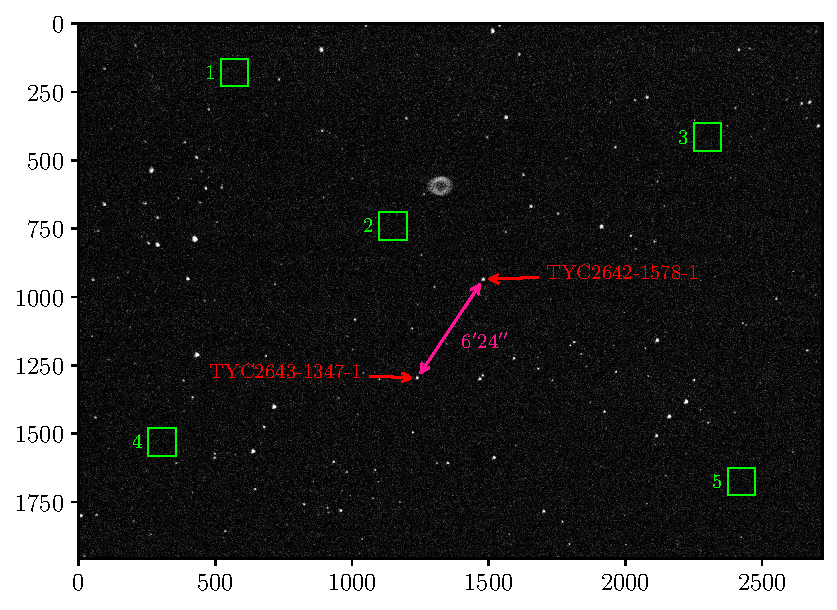
\includegraphics[width=\linewidth]{../markings}
		\caption{ستاره‌های انتخاب‌شده برای تبدیل واحد
			و شماره‌گذاری قطعه‌های «خالی» انتخاب‌شده برای محاسبه روشنایی زمینه.}
		\label{fig:markings}
	\end{figure}
	\section{نتایج}
	با جمع روشنایی پیکسل‌های داخل محدوده‌های «خالی» تصویر (یعنی محدوده‌هایی که به نظر می‌رسد ستاره‌ای در آن وجود
	ندارد) و تقسیم آن بر تعداد پیکسل‌های آن ناحیه و مقایسه قدر با قدر ستاره مرجع، قدر سطحی زمینه را بدست می‌آوریم.
	تصویر کاملاً یکنواخت نیست، بنابراین برای بدست آوردن عددی دقیق‌تر برای روشنایی زمینه، از پنج محدوده مختلف در
	بخش‌های متفاوت تصویر، دور از یکدیگر، استفاده کردیم که در شکل \ref{fig:markings} مشخص شده‌اند. ابعاد هر قطعه
	صد پیکسل در صد پیکسل است.
	\begin{table}[h!]
		\centering
		\caption{قدر سطحی زمینه عکس.}
		\begin{LTR}
		\begin{tabular}{|c|c|}
			\hline
			\rl{شماره محدوده} & قدر بر ثانیه کمانی مربع \\ \hline
			$1$ & $21.4$ \\ \hline
			$2$ & $21.5$ \\ \hline
			$3$ & $21.4$ \\ \hline
			$4$ & $21.7$ \\ \hline
			$5$ & $21.5$ \\ \hline
			$\text{میانگین}\pm\text{\rl{انحراف معیار}}$ & $21.5\pm0.1$ \\ \hline
		\end{tabular}
		\end{LTR}
	\end{table} 
\end{document}